\section{Auswertung}
\label{sec:Auswertung}

Zur Bestimmung der Ladung der Öltröpfchen werden Messungen für die Kondensatorspannungen
\begin{align*}
U_1 &= \SI{190}{\volt},\\
U_2 &= \SI{302}{\volt},\\
U_3 &= \SI{250}{\volt}
\end{align*}
durchgeführt.
Die Temperaturen der Messapparatur bestimmen sich aus den gemessenen Werten des Thermowiderstandes unter Verwendung der Tabelle \ref{tab:thermo} zu
\begin{align*}
R_1 &= \SI{1.71}{\mega\ohm},\\
T_1 &= \SI{32}{\celsius},\\
R_2 &= \SI{1.67}{\mega\ohm},\\
T_2 &= \SI{33}{\celsius}.\\
\end{align*}
Bei der Betrachtung der Werte fällt auf, dass vereinzelt eine starke Abweichung der Messzeiten während einer einzigen Messreihe aufgetreten ist.
Diese Messwerte können dementsprechend nicht verwendet werden.
Zudem werden die Messwerte verworfen, wenn die Bedingung
\begin{align*}
  v_{\text{ab}} - v_{\text{auf}} = 2 v_0
\end{align*}
nicht erfüllt wird.
Somit werden die in den Tabellen \ref{table:1} bis \ref{table:6} angegebenen Messwerte verwendet.
Von diesen Zeiten wird für jede Messreihe, also für jedes betrachtete Teilchen, der Mittelwert gebildet,
Der betrachtete Strecke beträgt jeweils $s = \SI{1}{\milli\metre}$, woraus sich mit den gemittelten Zeiten die Geschwindigkeiten $v_{\text{ab}}$ und $v_{\text{auf}}$ ergeben.

\begin{table}
    \centering
    \caption{Bestimmung der Schallgeschwindigkeit mittels Durchschallungs-Methode.}
    \label{tab:1}
    \sisetup{parse-numbers=false}
    \begin{tabular}{
	S[table-format=2.2]
	S[table-format=2.1]
	S[table-format=4.2]
	}
	\toprule
	{$h_{\text{zylinder}} \:/\: 10^{-3} \si{\metre}$}		& {$\increment t \:/\: 10^{-6} \si{\second} $}		& 
	{$c_\text{Acryl} \:/\: \si{\metre\per\second} $}		\\ 
	\midrule
    31.30 & 11.5 & 2709.96 \\
61.50 & 22.8 & 2697.37 \\
80.55 & 30.4 & 2645.32 \\

    \bottomrule
    \end{tabular}
    \end{table}


\input{build/Tabelle_2_texformat.tex}

\input{build/Tabelle_3_texformat.tex}

\input{build/Tabelle_4_texformat.tex}

\input{build/Tabelle_5_texformat.tex}

\input{build/Tabelle_6_texformat.tex}
\clearpage

%Von diesen Zeiten wird für jede Messreihe, also für jedes betrachtete Teilchen, der Mittelwert gebildet,
%Der betrachtete Strecke beträgt jeweils $s = \SI{1}{\milli\metre}$, woraus sich mit den gemittelten Zeiten die Geschwindigkeiten $v_{\text{ab}}$ und $v_{\text{auf}}$ ergeben.
\subsection{Einfache Bestimmung der Elementarladung}

Die daraus nach Formel \eqref{eqn:1} resultierenden Ladungen sind in Tabelle \ref{table:q} dargestellt.
Dabei wird die Beziehung
\begin{equation}
  E = \frac{U}{d},
\end{equation}
welche für das elektrische Feld $E$ eines Plattenkondensators gilt, ausgenutzt.
Die verwendeten Konstanten sind \cite{skript} \cite{chemie}
\begin{align*}
  \rho_{\text{Oel}}  &= \SI{886}{\kilo\gram\per\metre\tothe{3}},\\
  \rho_{\text{Luft}} &= \SI{1,1644}{\kilo\gram\per\metre\tothe{3}},\\
  g                  &= \SI{9,81}{\metre\per\second},\\
  d                  &= \SI{7,6250 \pm 0,0051}{\milli\metre},\\
\end{align*}
wobei die Viskosität $n$ von Luft je nach Temperatur aus dem Diagramm \ref{luft_n_shit} entnommen wird.
\input{build/Tabelle_q_texformat.tex}

Zusätzlich sind diese in Diagramm \ref{plot:1} dargestellt.
\begin{figure}
  \centering
  \includegraphics[height=8cm]{build/ladungen.pdf}
  \caption{Ermittelte Ladungen.}
  \label{plot:1}
\end{figure}

Wird nun der größte gemeinsame Teiler dieser Werte bestimmt, so ergibt sich ein ermittelter Wert für die Elementarladung von
\begin{align*}
  e_0 = \input{build/e_0.tex}.
\end{align*}

Die Avogadro-Konstante wird durch die Formel
\begin{equation}
  N_{\text{a}} = \frac{F}{e_0},
\end{equation}
mit der Faraday-Konstante $F = \SI{96485,3365}{\coulomb\per\mol}$ \cite{chemie}, beschrieben.
Dadurch wird die Avogadro-Konstante auf
\begin{align*}
  N_{a} = \input{build/N_a.tex}
\end{align*}
bestimmt.


\subsection{Bestimmung der Elementarladung mit Korrekturfaktor}

Um die Ladungen nach Formel \eqref{blubb} zu bestimmen, muss zunächst der Radius $r$ des Tröpfchens bekannt sein.
Jener wird über die Formel \eqref{blubbr}, mit den wie zuvor auch verwendeten Parametern, ermittelt.
Die Radien der in der Messreihe verwendeten Öltröpfchen sind in Tabelle \ref{tabella} einzusehen.

\input{build/Tabelle_r_texformat.tex}

Mit den Parametern \cite{skript} \cite{normaldruck}
\begin{align*}
  B &= 6,17\cdot 10^{-3}\text{Torr},\\
  p &= 1013,25\cdot10^2\si{\pascal}
\end{align*}
ergeben sich die somit neu bestimmten Ladungen aus Tabelle \ref{table:q_neu}, welche auch in Diagramm \ref{plot:2} dargestellt sind.

\input{build/Tabelle_q_neu_texformat.tex}


\begin{figure}
  \centering
  \includegraphics[height=8cm]{build/ladungen_neu.pdf}
  \caption{Korrigierte Ladungen.}
  \label{plot:2}
\end{figure}

Somit ergibt sich eine Elementarladung von

\begin{align*}
  e_{0,\text{neu}} = \input{build/e_0_neu.tex}
\end{align*}
und die Avogadro-Konstante beträgt nun
\begin{align*}
  N_{a,\text{neu}} = \input{build/N_a_neu.tex}.
\end{align*}



% % Examples
% \begin{equation}
%   U(t) = a \sin(b t + c) + d
% \end{equation}
%
% \begin{align}
%   a &= \input{build/a.tex} \\
%   b &= \input{build/b.tex} \\
%   c &= \input{build/c.tex} \\
%   d &= \input{build/d.tex} .
% \end{align}
% Die Messdaten und das Ergebnis des Fits sind in Abbildung~\ref{fig:plot} geplottet.
%
% %Tabelle mit Messdaten
% \begin{table}
%   \centering
%   \caption{Messdaten.}
%   \label{tab:data}
%   \sisetup{parse-numbers=false}
%   \begin{tabular}{
% % format 1.3 bedeutet eine Stelle vorm Komma, 3 danach
%     S[table-format=1.3]
%     S[table-format=-1.2]
%     @{${}\pm{}$}
%     S[table-format=1.2]
%     @{\hspace*{3em}\hspace*{\tabcolsep}}
%     S[table-format=1.3]
%     S[table-format=-1.2]
%     @{${}\pm{}$}
%     S[table-format=1.2]
%   }
%     \toprule
%     {$t \:/\: \si{\milli\second}$} & \multicolumn{2}{c}{$U \:/\: \si{\kilo\volt}$\hspace*{3em}} &
%     {$t \:/\: \si{\milli\second}$} & \multicolumn{2}{c}{$U \:/\: \si{\kilo\volt}$} \\
%     \midrule
%     \input{build/table.tex}
%     \bottomrule
%   \end{tabular}
% \end{table}
%
% % Standard Plot
% \begin{figure}
%   \centering
%   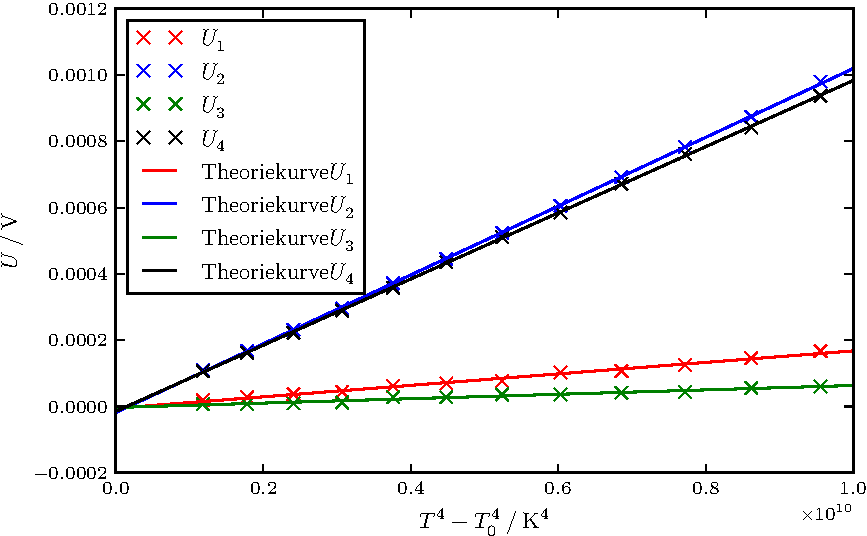
\includegraphics{build/plot.pdf}
%   \caption{Messdaten und Fitergebnis.}
%   \label{fig:plot}
% \end{figure}
%
% 2x2 Plot
% \begin{figure*}
%     \centering
%     \begin{subfigure}[b]{0.475\textwidth}
%         \centering
%         \includegraphics[width=\textwidth]{Abbildungen/Schaltung1.pdf}
%         \caption[]%
%         {{\small Schaltung 1.}}
%         \label{fig:Schaltung1}
%     \end{subfigure}
%     \hfill
%     \begin{subfigure}[b]{0.475\textwidth}
%         \centering
%         \includegraphics[width=\textwidth]{Abbildungen/Schaltung2.pdf}
%         \caption[]%
%         {{\small Schaltung 2.}}
%         \label{fig:Schaltung2}
%     \end{subfigure}
%     \vskip\baselineskip
%     \begin{subfigure}[b]{0.475\textwidth}
%         \centering
%         \includegraphics[width=\textwidth]{Abbildungen/Schaltung4.pdf}    % Zahlen vertauscht ... -.-
%         \caption[]%
%         {{\small Schaltung 3.}}
%         \label{fig:Schaltung3}
%     \end{subfigure}
%     \quad
%     \begin{subfigure}[b]{0.475\textwidth}
%         \centering
%         \includegraphics[width=\textwidth]{Abbildungen/Schaltung3.pdf}
%         \caption[]%
%         {{\small Schaltung 4.}}
%         \label{fig:Schaltung4}
%     \end{subfigure}
%     \caption[]
%     {Ersatzschaltbilder der verschiedenen Teilaufgaben.}
%     \label{fig:Schaltungen}
% \end{figure*}
